\chapter{Evaluation}
In this chapter we explain how we used the system described in \Cref{sec:approach} to evaluate its performance.
First, we review the results of the \ac{mcts} approach in \Cref{sec:eval:mcts}.
Followingly, we evaluate if we can use the results of the \ac{mcts} approach to learn to generate good schedules with supervised learning methods in \Cref{sec:eval:supervised}.

\section{Hardware selection}
\label{sec:eval:hw}
There are different aspects in choosing the hardware for our experiments.
Two aspects must be given that a processor makes sense.
The first is, that it is supported in LLVM because our whole approach is based on LLVM and we use the LLVM instruction scheduler as a baseline.
Secondly, we limit the hardware choice to processors that implement superscalar pipelines (see \Cref{sec:bg:superscalar-cpu}) because these are used in most modern processors.

However, we consider more aspects regarding the hardware to be important.
The most interesting one is if the superscalar pipeline is implemented as in-order or out-of-order.
While the former comes with no restrictions for our experiments, the latter is able to reschedule instructions during execution in hardware.
Followingly, it is interesting to see how the out-of-order model influences the performance of our approach.

Additionally, to show the versatility of our approach, it is interesting to choose different types of processors.
There exist classical \acp{cpu}, Edge \acp{cpu}, accelerator cards (\eg Graphical Processing Units (GPU), Vector Processing Units, and Intelligence Processing Units (IPU)), and others.

With these aspects in mind we choose to use:
\begin{itemize}
    \item \textbf{Arm Cortex-A53:} This processor is a edge \ac{cpu} and implements an in-order superscalar pipeline based on the AArch64 architecture.
    An edge device that uses it is the Raspberry Pi 3 Model B.
    We use this device for our experiments with a Ubuntu 20.04.
    \item \textbf{\aurora:} This processor is interesting because it implements an out-of-order superscalar pipeline. 
    Additionally, it is an vector processing accelerator card, and thus a different type of processor that is installed via a PCI-Express connection.
\end{itemize}


\section{Approach Validation}
\label{sec:eval:validation}
Before starting to optimize a process, it is useful to validate that there is potential for any optimizations.
Therefore, we show, that different instruction schedules can indeed have different runtimes on our target hardware.
The approach of this experiment is differs from the other experiments because it is an early experiment that took place before our pipeline was developed.
\todo{Is this sentence useful /okay?}

% select longest bb per benchmark
% longest might have the most possible schedule, so more variation in the random schedules
\Cref{sec:approach:dataset} describes the selection of benchmarks from the LLVM Test Suite.
For this experiment we select one basic block per benchmark, for which we modify its instruction schedule.
For the selection of basic blocks we use the heuristic that balances between the most executions and the longest basic blocks, which is discussed in \Cref{sec:approach:basicblock:selection}.
A high number of instructions in a basic block is typically a good indicator for a high number of possible instruction schedules for that basic block. 
A high number of executions ensures that the basic block has a high impact on the runtime of the function that it contains.

% measure the function runtime
% we measure the runtime of the function (implemented llvm passes)
% talk about impact on measurements.
We executed this experiment in a early stage and did not have a basic block extraction pipeline nor means to measure the execution time of a single basic block.
Therefore, we must execute the whole benchmark with the modified instruction schedule of a single basic block.
However, measuring the runtime of the whole benchmark, includes the execution of much overhead code, that we are not interested in.
Thus, we measure the runtime of the function that contains the basic block of interest.
This corresponds to the third method in \Cref{fig:approach:runtime_scopes}.

We implement a pass for the LLVM optimizer, to measure the runtime of a single function.
\todo{Put into approach chapter?}
The pass searches for the function that contains the selected basic block.
Then, it injects calls to the timer functions of the C++ standard library (\lstinline|std::high_resolution_clock::now|).
The calls are injected at the beginning of the given function and right before the return statement.
It injects a compilation-unit-wide global variable, and stores the measurements into this variable.
In the destructor of that compilation-unit, the pass injects code to print all the measurements.

% generate 10 different random schedules 
% do that twice
To generate different different instruction schedules, we choose the simple approach of generating random schedules.
Our random instruction scheduler works on top of a basic list scheduler.
This means, that the list scheduler selects the instructions that are ready for scheduling, and our random scheduler randomly selects one of them.
This is done until no more instructions are left.
We set the seed of the random number generator for reproducibility.

We generate instruction schedules with the seeds 0-10 for each selected basic block, \ie we generate 11 instruction schedules per basic block.
The basic block of interest might execute multiple times in the measured function for reasons discussed in \Cref{sec:approach:runtime-measurement-unit}.
We choose the shortest measured runtime per benchmark run, to ensure that we use the same execution path in our measurements.
To check that the runtime measurements are reproducible, we run the each generated instruction schedule two times.

% evaluate
We have run this experiment on the two processors described in \Cref{sec:eval:hw}.
\Cref{fig:eval:rndm:aarch64} shows a selection of experiment results.
The plots show the runtimes grouped by the different seeds for the random instruction scheduler.
Runtimes that differ between two runs more than 5\% are marked as outliers and plotted in gray.
\Crefrange*{fig:eval:rndm:aarch64:a}{fig:eval:rndm:aarch64:d} show examples where different runtimes are clearly observable for different instruction schedules.
However, this was not always observable.
\Cref{fig:eval:rndm:aarch64:e} and \Cref{fig:eval:rndm:aarch64:f} show examples where no differnce in the runtime was observable.
The average coeffecient of variation over the basic blocks is 0.035.
In summary, we see that different instruction schedules can generate measurable differences in the runtime.
This means that there is potential for improvements.
\begin{figure}
    \begin{subfigure}{0.0325\textwidth}\caption{}\label{fig:eval:rndm:aarch64:a}\end{subfigure}
    \begin{subfigure}{0.44\textwidth}
        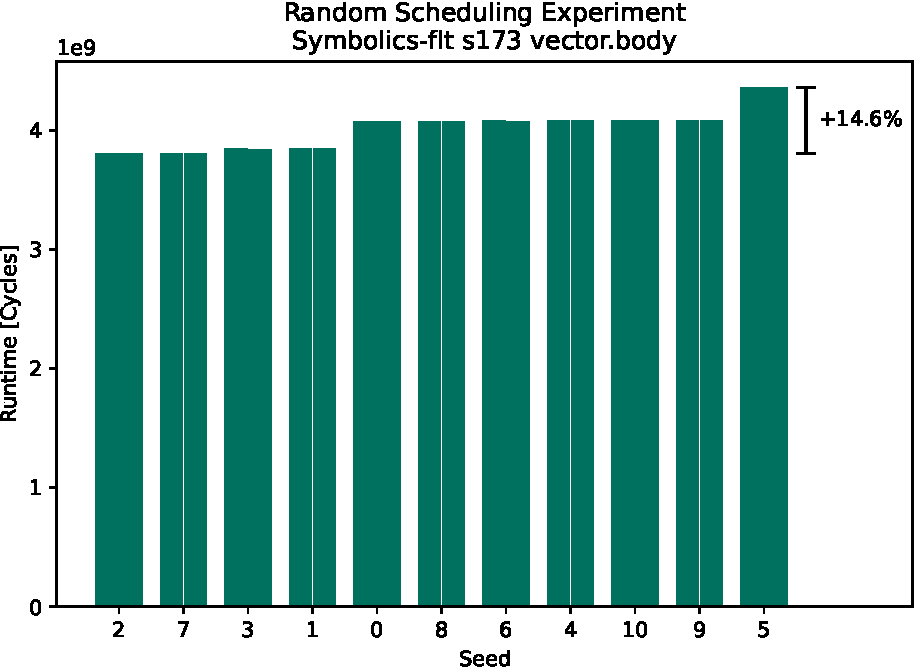
\includegraphics[width=\textwidth]{img/random-scheduling-experiment-pi-collected/Symbolics-flt-crop.pdf}
    \end{subfigure}
    \hfill
    \begin{subfigure}{0.0325\textwidth}\caption{}\label{fig:eval:rndm:aarch64:b}\end{subfigure}
    \begin{subfigure}{0.44\textwidth}
        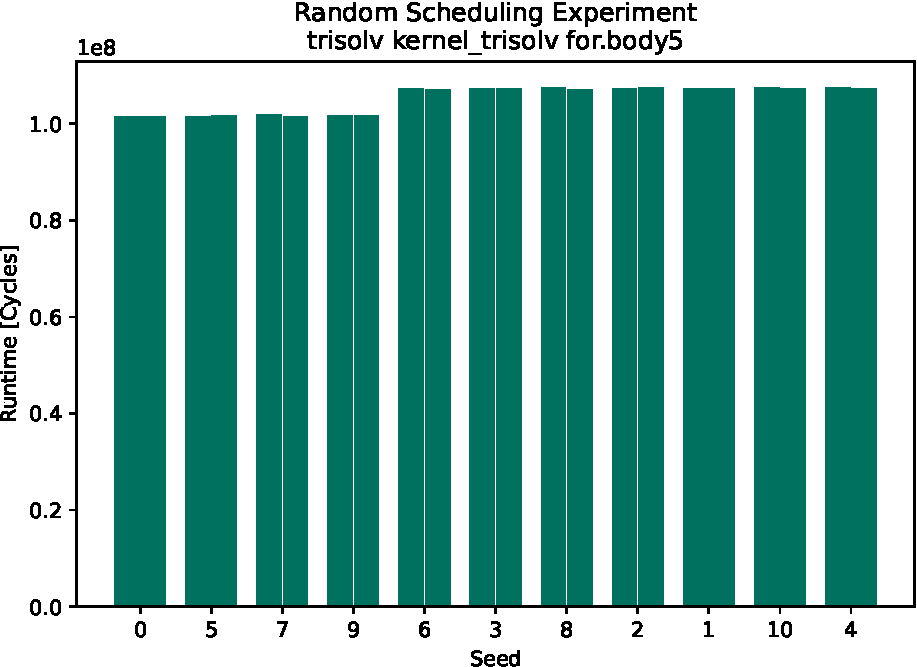
\includegraphics[width=\textwidth]{img/random-scheduling-experiment-pi-collected/trisolv-crop.pdf}
    \end{subfigure}

    \vspace{0.5cm}
    \begin{subfigure}{0.0325\textwidth}\caption{}\label{fig:eval:rndm:aarch64:c}\end{subfigure}
    \begin{subfigure}{0.44\textwidth}
        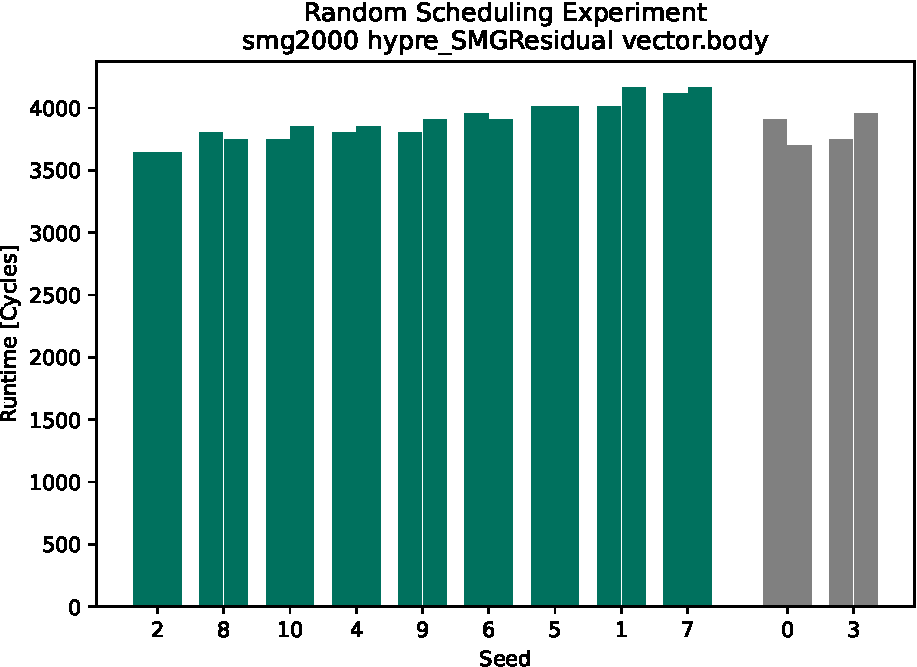
\includegraphics[width=\textwidth]{img/random-scheduling-experiment-pi-collected/smg2000-crop.pdf}
    \end{subfigure}
    \hfill
    \begin{subfigure}{0.0325\textwidth}\caption{}\label{fig:eval:rndm:aarch64:d}\end{subfigure}
    \begin{subfigure}{0.44\textwidth}
        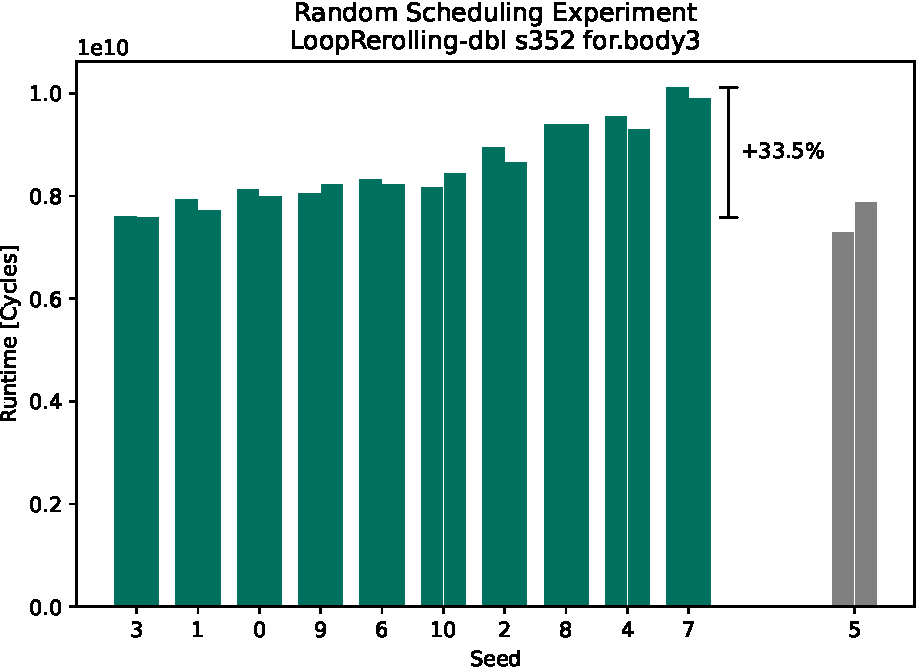
\includegraphics[width=\textwidth]{img/random-scheduling-experiment-pi-collected/LoopRerolling-dbl-crop.pdf}
    \end{subfigure}

    \vspace{0.5cm}
    \begin{subfigure}{0.0325\textwidth}\caption{}\label{fig:eval:rndm:aarch64:e}\end{subfigure}
    \begin{subfigure}{0.44\textwidth}
        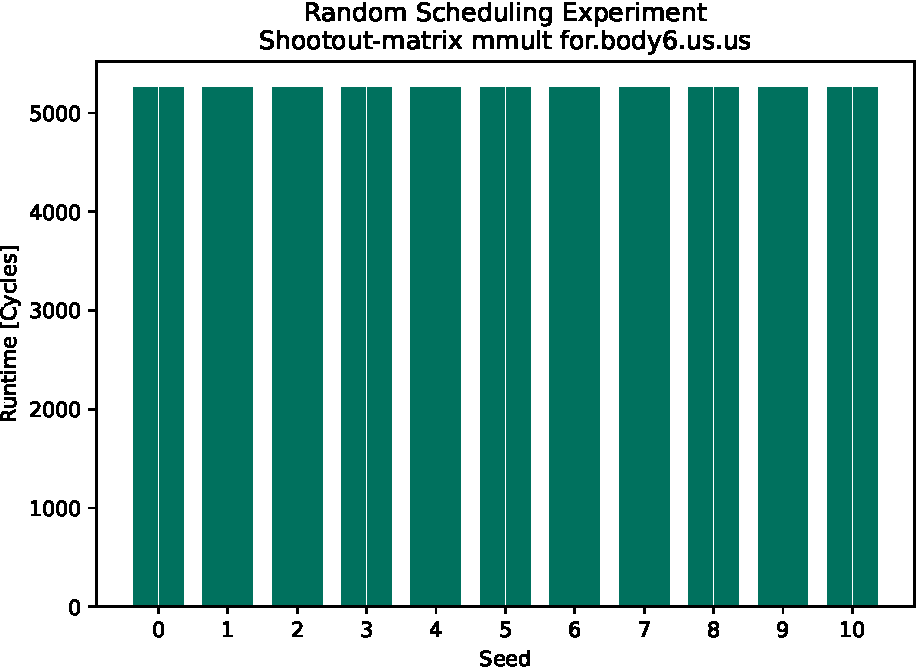
\includegraphics[width=\textwidth]{img/random-scheduling-experiment-pi-collected/Shootout-matrix-crop.pdf}
    \end{subfigure}
    \hfill
    \begin{subfigure}{0.0325\textwidth}\caption{}\label{fig:eval:rndm:aarch64:f}\end{subfigure}
    \begin{subfigure}{0.44\textwidth}
        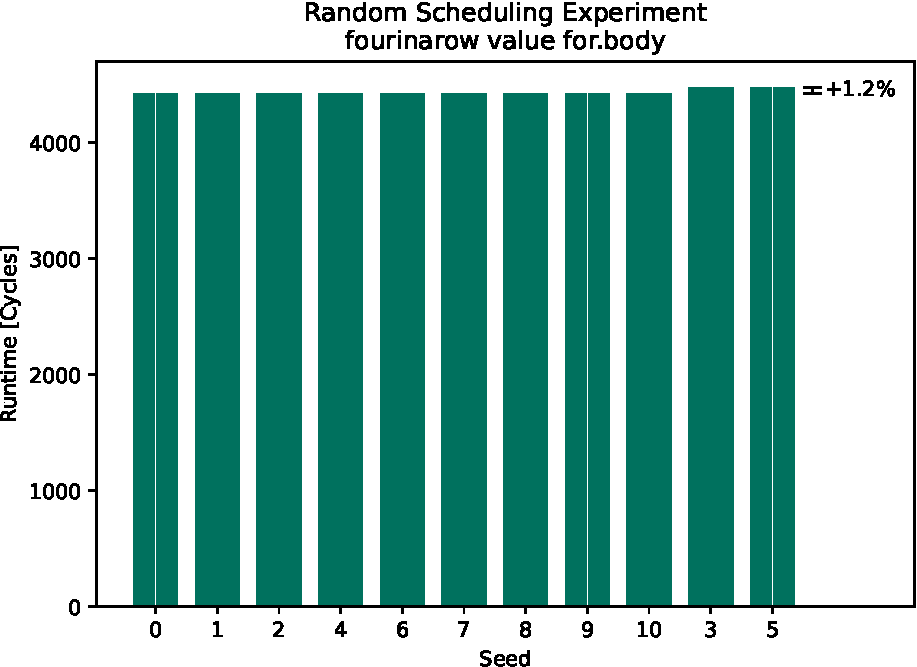
\includegraphics[width=\textwidth]{img/random-scheduling-experiment-pi-collected/fourinarow-crop.pdf}
    \end{subfigure}

    \caption[Random Scheduling Experiment on AArch64]{Random Scheduling Experiment on AArch64:
    The bars show the runtime of a function with a random instruction schedule.
    The two runs of the instruction schedule are grouped together.
    The distance measure represents the longest execution time relative to the shortest execution time.
    Two runs that differ more than 5\% are marked as outliers and plotted in gray.}
    \label{fig:eval:rndm:aarch64}
\end{figure}

\Cref{fig:eval:rndm:aurora} shows a similar selection for the same experiment on the \aurora processor.
We can observe a similar outcome of the experiment.
However, as this processor cannot be interrupted by the \ac{os}, the runtimes are more stable between two runs.
No measurements in the whole example where marked as outliers.
The average coeffecient of variation over the basic blocks is 0.046.
In summary, we observe potential for optimizations on this processor.
\begin{figure}
    \begin{subfigure}{0.0325\textwidth}\caption{}\label{fig:eval:rndm:aurora:a}\end{subfigure}
    \begin{subfigure}{0.44\textwidth}
        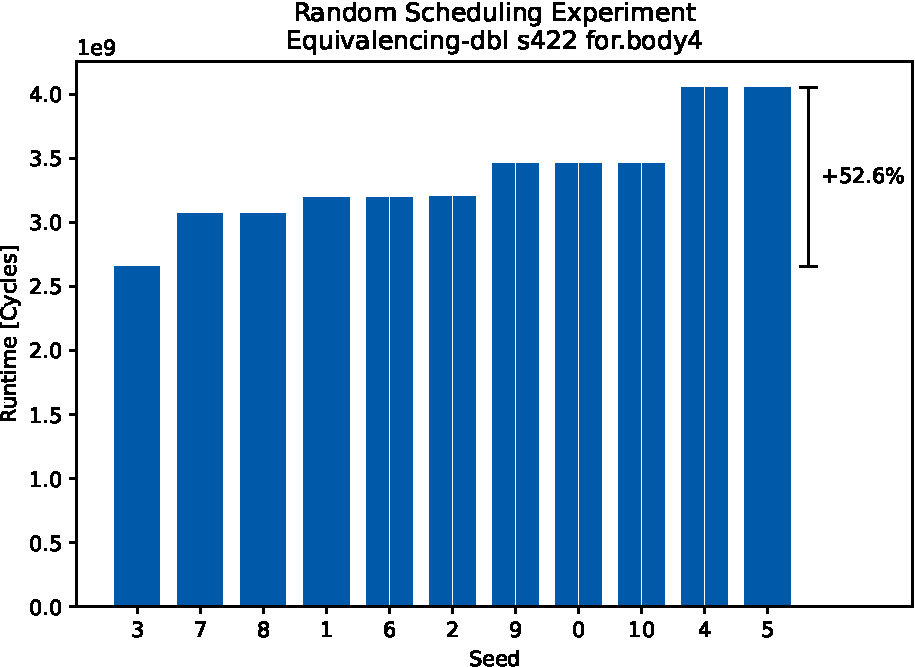
\includegraphics[width=\textwidth]{img/random-scheduling-experiment-aurora-collected/Equivalencing-dbl-crop.pdf}
    \end{subfigure}
    \hfill
    \begin{subfigure}{0.0325\textwidth}\caption{}\label{fig:eval:rndm:aurora:b}\end{subfigure}
    \begin{subfigure}{0.44\textwidth}
        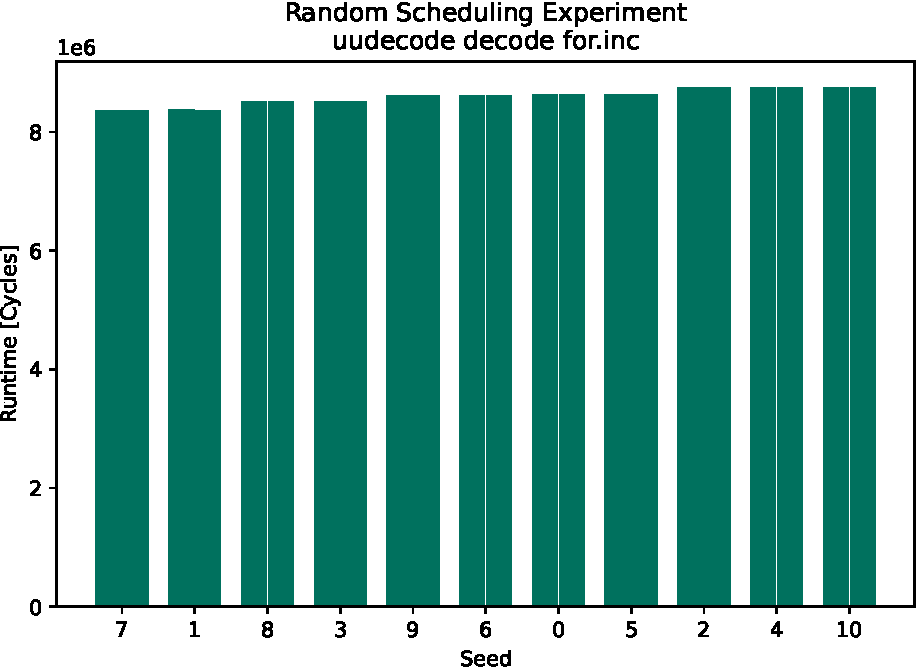
\includegraphics[width=\textwidth]{img/random-scheduling-experiment-aurora-collected/uudecode-crop.pdf}
    \end{subfigure}

    \vspace{0.5cm}
    \begin{subfigure}{0.0325\textwidth}\caption{}\label{fig:eval:rndm:aurora:c}\end{subfigure}
    \begin{subfigure}{0.44\textwidth}
        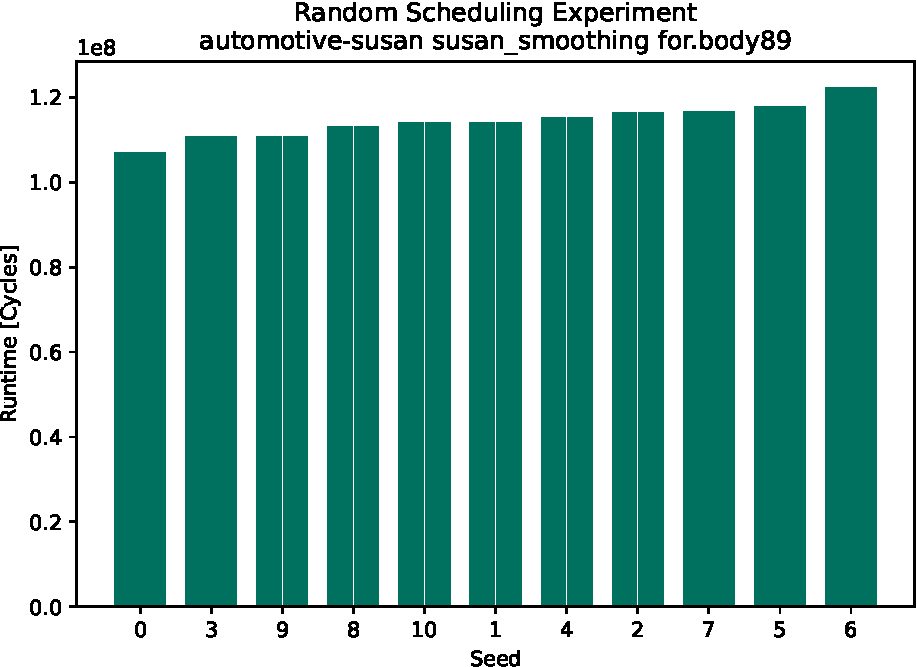
\includegraphics[width=\textwidth]{img/random-scheduling-experiment-aurora-collected/automotive-susan-crop.pdf}
    \end{subfigure}
    \hfill
    \begin{subfigure}{0.0325\textwidth}\caption{}\label{fig:eval:rndm:aurora:d}\end{subfigure}
    \begin{subfigure}{0.44\textwidth}
        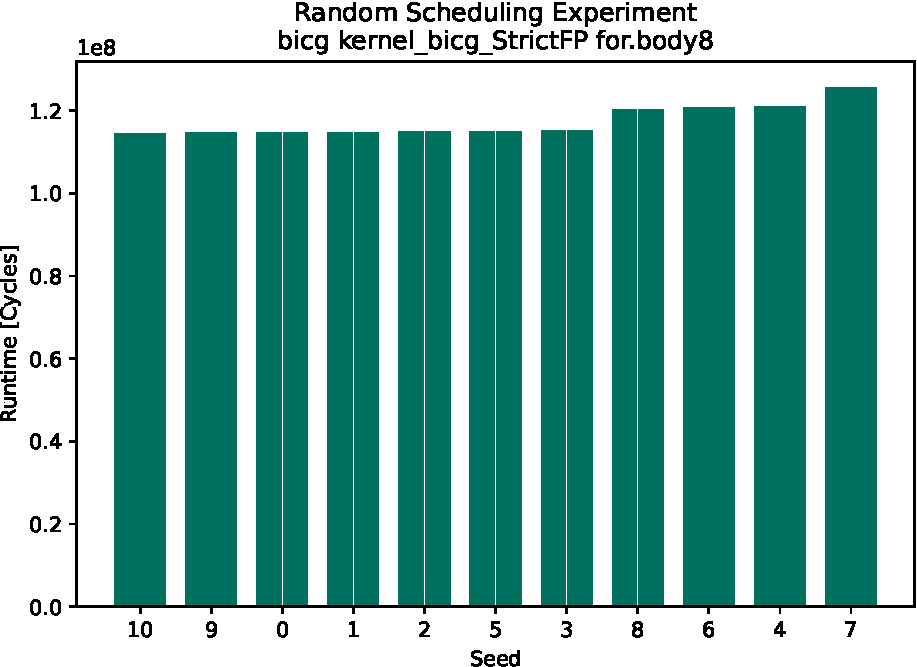
\includegraphics[width=\textwidth]{img/random-scheduling-experiment-aurora-collected/bicg-crop.pdf}
    \end{subfigure}

    \vspace{0.5cm}
    \begin{subfigure}{0.0325\textwidth}\caption{}\label{fig:eval:rndm:aurora:e}\end{subfigure}
    \begin{subfigure}{0.44\textwidth}
        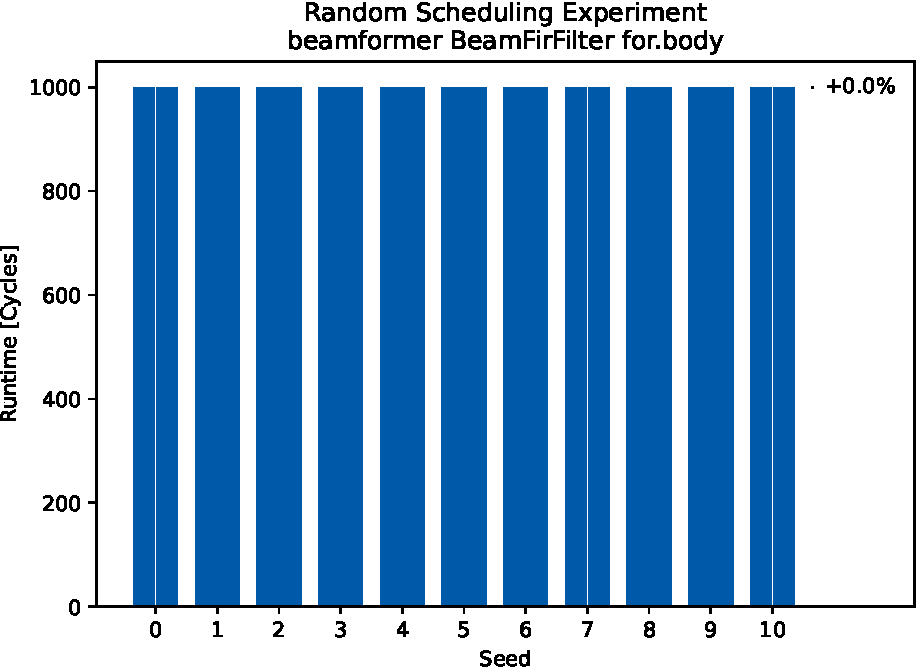
\includegraphics[width=\textwidth]{img/random-scheduling-experiment-aurora-collected/beamformer-crop.pdf}
    \end{subfigure}
    \hfill
    \begin{subfigure}{0.0325\textwidth}\caption{}\label{fig:eval:rndm:aurora:f}\end{subfigure}
    \begin{subfigure}{0.44\textwidth}
        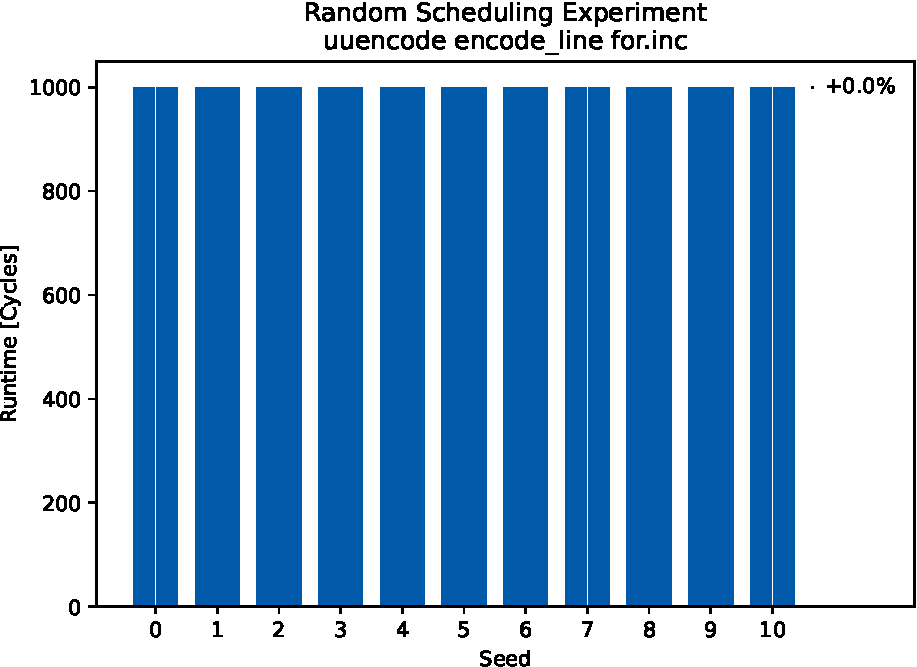
\includegraphics[width=\textwidth]{img/random-scheduling-experiment-aurora-collected/uuencode-crop.pdf}
    \end{subfigure}

    \caption[Random Scheduling Experiment on \aurora]{Random Scheduling Experiment on \aurora:
    The bars show the runtime of a function with a random instruction schedule.
    The two runs of the instruction schedule are grouped together.
    The distance measure represents the longest execution time relative to the shortest execution time.
    Two runs that differ more than 5\% are marked as outliers.
    However, this processor did not produce any outliers in our experiment.}
    \label{fig:eval:rndm:aurora}
\end{figure}

There are multiple possible reasons that would cause equal measurements in this experiment.
We must differntiate between reasons which mean that different instruction schedules have no effect on the runtime of the basic block and reasons that have its origin in the experiment setup.
We cannot do anything about the former.
Actually, the motivation for this experiment was to verify, that the former reasons do not dominate all the instruction schedules.
There are multiple possibilities for the latter reasons, that have ther origin in the experiment setup:
\begin{itemize}
    \item The basic block for which we manipulate the instruction schedule might have a low influence on the runtime of the function.
        We tried to minimize this effect by choosing basic blocks that are often executed.
    \item Our random instruction scheduler works on top of LLVM.
        LLVM makes, in this stage of the back-end, still use of pseudo instruction that are not represented in the binary.
        This means that schedules that we see as different schedules, might actually not differ in the binary.
    \item There are short functions with a short execution time.
        We observed few changes in the runtime when the measured execution time is below 10,000 processor cycles.
        The underlying timer of the C++ standard library might not be able to measure such short time periods.  
\end{itemize}
However, the experiment is still valid, because we show that we are able to influence the runtime by manipulating the instruction schedules.

In summary, we observe different runtimes for different instruction schedules and the results are reproducible over multiple runs.
This is not true for all basic blocks, but the goal of this experiment was to show the existence of an effect of the instruction schedule on the runtime.
These results motivate the further research on optimizing instruction schedules for these two processors.

\section{MCTS Schedule Search}
\label{sec:eval:mcts}
% Goal of the experiment
We pursue two goals with this experiment.
One is to search instruction schedules that perform better than our baseline.
As our baseline, we choose the LLVM default instruction scheduler, which is defined in the architecture specific compiler back-end.
The second goal is to build a dataset that we can use for our supervised learning approaches.
As a side-effect, we will generate an upper limit for the supervised models.

% What do we do in this experiment
For each basic block under consideration, we first measure the runtime of the basic block compiled with the LLVM default instruction scheduler for the given processor.
Next, we generate an instruction schedule in each \ac{mcts} iteration.
We compile the instruction schedule into an executable format (\Cref{sec:approach:bbisolation}) and execute it to measure the runtime of the basic block of interest (\Cref{sec:approach:datageneration:runtime_methods}).
We train the \ac{mcts} model with the score computed by \Cref{eqn:approach:mcts-score} and start the next iteration to train the \ac{mcts} model.
This way, we generate many instruction schedules per basic block, each evaluated with a score based on their execution time relative to the default instruction schedule.

% Baseline

% How many (and which) BBs do we use
To have a large number of instruction schedules available for our supervised learning methods, we select 20,032 basic blocks from the LLVM Test Suite. \todo{describe how we got the basic blocks}
We generate one \ac{mcts} model for each basic block.
For this experiment, we have selected the longest basic blocks in the dataset.
The number of executions is not relevant in this experiment because we isolate the basic block and measure their specific runtime on the target hardware.
A high number of instructions in the basic blocks helps to avoid trivial scheduling situations.

% Number of steps to outroll the MCTS tree
The experiment is time consuming because of the high number of basic blocks and the expensive compilation and runtime measurements.
We have to terminate the experiment at some point.
After 200 iterations, we have seen that we get a speedup for many basic blocks.
Therefore, we run the \ac{mcts} model for each basic block for 200 iterations.
The experiment execution took 5 weeks for the AArch64, and 3 weeks for the \aurora.

% Exploration vs Exploitation balance weight
% WE DID NOT DESCRIBE THE FORMULAR NOWHERE

% Caching of schedules to detect duplicates
Due to the high cost of the compilation and runtime measurements, we try to avoid these steps as much as possible.
The instruction schedule generation is done in two steps:
We generate the schedule in the LLVM back-end format that can still contain pseudo instructions, and the remaining steps in the LLVM back-end transform this into assembly instructions.
After the removal of pseudo instructions, it can happen that two equal assembly instruction schedules are generated from two different instruction schedules in the LLVM back-end format.
Therefore, we cache the measured runtimes with the hashes of the instruction schedules.
Whenever we already executed a instruction schedule with the same hash, we reuse their measured runtimes.

% Performance: Summary of the excel tables
For the AArch64 we were able to run this experiment on 14,217 basic blocks.
Due to some errors, we measured an unrealistic speed up for some basic blocks.
So, all speed ups greater than a factor of 2 are marked as outliers.
That leaves us with 14,162 valid instruction schedules for the AArch64 processor.
\Cref{tbl:eval:mcts} summarizes the results.
We find better performing instruction schedules for 54.79\% of these basic blocks.
In only 8.24\% of the basic blocks, we did not find an instruction schedule that performed least as good as the LLVM generated one.
On average, we increase the runtime performance of the basic blocks by 8.35\%.
\begin{table}
    \centering
    \begin{tabular}{@{}lrr@{}}
        \toprule
        & \multicolumn{2}{c}{Processor} \\
        \cmidrule{2-3}
        Performance & AArch64 & \aurora \\
        \midrule
        \tblsection{Absolute} && \\
        \tblitem{Better than baseline}    & 54.79\% (7759) & 31.73\% (1349) \\
        \tblitem{Same as baseline}        & 36.97\% (5236) & 53.00\% (2253) \\
        \tblitem{Worse than baseline}     &  8.24\% (1167) & 15.27\%  (649) \\
        \tblsection{Runtime} && \\
        \tblitem{Mean Speed Up} & 8.35\% & 0.30\% \\
        \bottomrule
    \end{tabular}
    \caption[Results of the \ac{mcts} Approach]{Results of the \ac{mcts} approach. The \ac{mcts} approach was very successful on the AArch64 processor. We found better instruction schedules for more than the half of the basic blocks.
    On the \aurora, we are on par with the baseline for half of the basic blocks and fou nd better instruction schedules for a third of the basic blocks.}
    \label{tbl:eval:mcts}
\end{table}

We executed this experiment for 4,253 basic blocks on the \aurora processor.
The lower number of basic blocks is caused by hardware and time limitations.
Only two outliers are generated during this experiment, which results in 4,251 valid basic blocks.
See \Cref{tbl:eval:mcts} for the summarized results.
For this processor, our \ac{mcts} approach found better instruction schedules for 31.73\% of the basic blocks.
In 15.27\% of the basic blocks only worse instruction schedules were found by our model.
The average speed up of the basic blocks is 0.30\%.

% In-order vs OoO discussion (Speed Up vs BB length)
The results could still change in favor of the \aurora processor if we run this experiment on more basic blocks.
However, the result that the performance on this processor is worse than on the AArch64 processor was expected.
The reason is, that the \aurora is an out-of-order processor, and the AArch64 processor is an in-order processor.
Consequently, the \aurora might reschedule the instruction in hardware when it detects problems with the instruction schedule.
Thus, it does not depend on good instruction schedules as the AArch64 processor.

We showed with this experiment that we are able to find better instruction schedules for both our selected processors.
However, our search for instruction schedules was more successful for the AArch64 processor, as does no rescheduling in hardware.

\section{Supervised Schedule Generation}
\label{sec:eval:supervised}
As discussed, the \ac{mcts} approach is not usable for production systems because of its long runtime.
We use another approach for inference here, by using the generated dataset.
First we evaluate the nearest neighbor model, and then the parametric models.

The dataset that we use for our supervised models is based on the results of the \ac{mcts} approach (\Cref{sec:eval:mcts}).
We split this dataset into a training set with 80\% randomly selected data points and a test set with the remaining 20\%.
\Cref{fig:eval:datasets} illustrates the usage of the created datasets.
\begin{figure}
    \centering
    \tikzstyle{defaultnode} = [text centered, align=center, font=\footnotesize\accentfont, rectangle, rounded corners, draw=black, minimum height=1cm, minimum width=2.5cm]
    \tikzstyle{arrow} = [thick,->,>=stealth,-{Latex[scale=1.2]}, font=\footnotesize\accentfont]
    \begin{tikzpicture}
        \node (bb)              [defaultnode] at ( 0,1) {Basic Blocks};
        \node (bbe)             [defaultnode] at ( 4.5,1) {Basic Blocks \\ + \\ Evaluated \\ Instruction Schedules};
        \node (training-set)    [defaultnode] at ( 8.5,2) {Training Set};
        \node (test-set)        [defaultnode] at ( 8.5,0) {Test Set};
        \node (model)           [defaultnode] at (13,2) {Supervised \\ Model};
        \node (eval)            [defaultnode] at (15.5,0) {Supervised \\ Evaluation};

        \draw [arrow] (bb) -- node [midway,above] {MCTS} (bbe);
        \draw [arrow] (bbe) |- node [midway,above] {80\%} (training-set);
        \draw [arrow] (bbe) |- node [midway,below] {20\%} (test-set);
        \draw (training-set) -- node [midway,above=0.4cm] {\footnotesize\accentfont Supervised} (model);
        \draw [arrow] (training-set) -- node [midway,above] {Training} (model);
        \draw [arrow] (test-set) -- node [midway,below] {Model Inference} (eval);
        \draw [arrow] (model) |- (eval);
    \end{tikzpicture}
    \caption[Overview over the used Dataset]{Overview over used datasets. The supervised model is one from \Cref{sec:eval:supervised}.}
    \label{fig:eval:datasets}
\end{figure}

The goal of this experiment is to see if we can generate well performing instruction schedules without auto-tuning methods.

\subsection{Nearest Neighbor Model}
\begin{table}
    \centering
    \begin{tabular}{@{}lrr@{}}
        \toprule
        & \multicolumn{2}{c}{Processor}\\
        \cmidrule{2-3}
        Supervised Model & AArch64 & \aurora \\
        \midrule
        Nearest Neighbor & \textbf{1.38\%} & -3.03\% \\
        \tblsection{Support Vector Regression} && \\
        \tblitem{Balanced + Clustered} & -1.14\% & -3.53\% \\
        \tblitem{Balanced} & -1.18\% & -3.20\% \\
        \tblitem{Clustered} & -1.45\% & \textbf{-2.90\%} \\
        \tblsection{Neural Network} && \\
        \tblitem{Balanced + Clustered} & -0.48\% & -4.19\% \\
        \tblitem{Balanced} & -0.19\% & -3.19\% \\
        \tblitem{Clustered} & -0.47\% & -3.31\% \\
        \bottomrule
    \end{tabular}
    \caption[Performance of our Supervised Models]{Performance of our supervised models relative to the baseline:
    This table shows the mean speedup on the test set with our applied supervised learning models.
    Our nearest neighbor model performed best on the AArch64. 
    It is the only model that generated a positive mean speedup.
    On the \aurora, the SVR model with clustered instructions performed best.
    However, it is still worse than the baseline.}
    \label{tbl:eval:supervised-perf}
\end{table}

We use a big map structure to quickly search our dataset for similar scheduling situations.
The details of this approach are explained in \Cref{sec:app:nearest-neighbor}.
This model is then integrated into the LLVM compiler framework, and we use it to compile our basic blocks in the test set.

The instruction schedules that we compiled with this nearest neighbor model for the AArch64 processor performed better than the baseline instruction scheduler from LLVM.
The measured runtimes for the basic block are 1.38\% shorter.
On the \aurora processor however, the measured runtimes are 3.03\% slower than the basic blocks compiled with the baseline instruction scheduler (see \Cref{tbl:eval:supervised-perf}).

\subsection{Parametric Machine Learning Models}
The parametric models need, an additional data transformation bring it into the form \Cref{eqn:approach:regression-mapping}.
This results in a dataset of 4.9 million data points for the AArch64 architecture, and 1.3 million data points for the \aurora architecture.
We have to added two variations to the parametric approaches which we describe in the next paragraphs.
All approaches are run once with both variations and additionally with only one of the approaches, to see their effect.

% \subsubsection{Instruction Clustering}
There are many similar instructions in the instruction sets of the two processors.
To reduce the dimensionality and simplify the dataset, we cluster some instructions into an alias instruction.
For example, the addition instructions \lstinline|ADDWri| and \lstinline|ADDXri| of the AArch64 architecture are clustered into the same cluster.
These two instructions only differ in that one takes 32-bit values and the other 64-bit values.
See \Cref{appendix:instr-clusters} for exact clusterings.

% \subsubsection{Dataset Balancing}
Further, we balance our dataset in the target dimension.
The distribution of target values in our dataset follows a normal distribution.
However, this can be problematic because, the model might only learn to predict the mean in any situation.
Therefore, we duplicate samples whose target value is further away from the mean and delete samples whose target value is very close to the mean.
% We sort the dataset into 40 histogram bins.
% In order to not distort the dataset too much, we delete at most 50\% of the samples in a histogram bin and do not increase the number of occurances of a sample to more than 30 times.
\todo{How exactly}
This way we were able to generate a dataset that has a distribution that is closer to an equal distribution.
\begin{figure}
    \centering
    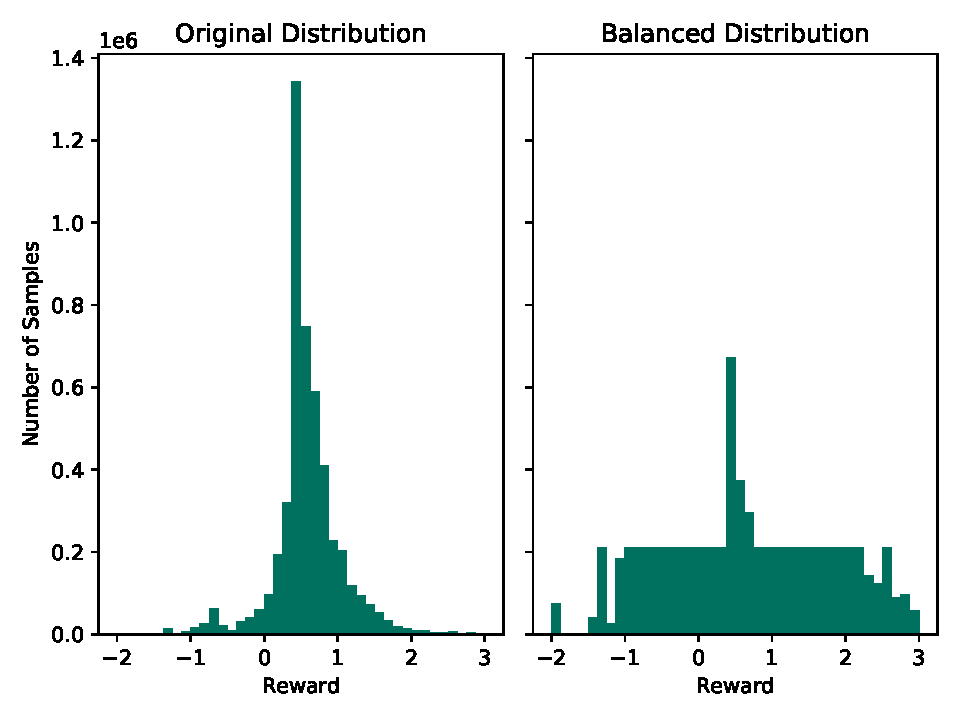
\includegraphics[width=0.75\textwidth]{img/balanced-supervised-dataset-rpi.pdf}
    \caption[Balancing for the AArch64 Dataset]{Balancing for the AArch64 dataset. 
    We duplicate samples with a reward further away from the distribution mean, and delete some samples that are close to the mean.}
    \label{fig:eval:balanced-dataset}
\end{figure}
\Cref{fig:eval:balanced-dataset} illustrates the effect on the distribution of the AArch64-dataset.
The effect for the \aurora dataset is similar.

\subsubsection{Support Vector Regression}
\label{sec:eval:svm}
\acp{svm} have long runtimes when trained with many data points.
We reduced this by randomly selecting 200,000 data points for our model training.

For the AArch64 processor, the average runtime of the instruction schedules generated by this model is between 1.14\% and 1.45\% worse than the runtime of the baseline.
This is the worst result of the parametric models on this processor.

On the \aurora however, we found the best working parametric model to be the \ac{svr} approach combined with clustered instructions.
But it performs still worse than on the AArch64 processor.

Regarding the effects of the dataset balancing and instruction clustering, we see no clear effect.
For the AArch64 processor, the experiments with the balanced datasets perform better.
However, the effect is reversed for the \aurora.
Here, the dataset balancing negatively influenced the performance.

\subsubsection{Neural Network}
\label{sec:eval:nn}
For training the neural network, we use the early stopping scheme.
Once the loss does not improve once for at least $10^{-6}$ in the last 10 epochs, we abort the training.
Therefore, the dataset is split into another training and validation set with a 85/15 split.

The results on the AArch64 processor performs better than the \ac{svr} approach.
With the balanced dataset, we get close to the baseline performance.
However, this approach performs still worse than the baseline.

On the \aurora, the neural network approach performed the worst.
We can also see, that the approach performed the worst with the dataset balancing and the instruction clustering together.


\section{Summary}
The best supervised learning model that we have found is the nearest neighbor approach on the AArch64 processor.
In fact, it is the only one that performed better than the baseline instruction scheduler.
Close to the baseline performance gets the neural network that was trained with the balanced dataset.

For the two dataset variations where we balanced the dataset and clustered similar instructions, we can see that the balancing was helping.
Compare \Cref{tbl:eval:mcts} to see that the models trained with the balanced dataset performed better than with the clustered dataset in three out of four cases.
It even performed better in three out of four cases than the approach with balanced and clustered dataset, and in the one other case it is very close.
So the balancing helped performance wise, and the clustering had a negative influence on the performance.
It seems, that it indeed is important to differenctiate between instructions that only differ in small aspects like the bit width. 

We have seen that our supervised approaches have all worked better on the AArch64 processor.
This was expected due to the smaller dataset and thus the worse average speedup in the \ac{mcts} approach for the \aurora processor.
\Cref{tbl:eval:mcts} shows that the \aurora processor only achieved a 0.30\% speedup in the \ac{mcts} approach.
This value can be seen, as a upper limit for the supervised learning approaches because they are based on the results of the \ac{mcts} approach.

Another important effect, why the approach was not that successful on the \aurora is that it has a out-of-order pipeline.
This means it reschedules the instructions during execution in hardware, so we do not know what is actually executed.
We expected that we would see worse performance on out-of-order hardware.  

Compare speedup with complexity of the problem (number of possible schedulings) vs speedup

Compare CPU Architectures, In-Order vs Out-Of-Order (\url{https://en.wikipedia.org/wiki/Out-of-order_execution})
Here, check speedup vs basic block length, to see if ooo processors perform worse on long basic blocks where it can't see too many instructions ahead

Might be interesting for the discussion: \url{http://www.irisa.fr/alf/downloads/PMA/p241-mcfarlin.pdf}

Mean vs. Median discussion in runtime measurements

\begin{itemize}
    \item Hardware
    \begin{itemize}
        \item Arm Cortex-A53
        \item NEC Aurora
    \end{itemize}
\end{itemize}



Run \ac{mcts} more iterations, because the rest of the schedules still contain many random decision and we can see, that a single decision can make a big difference.
